    \documentclass[letterpaper, 11 pt]{article}
\usepackage[utf8]{inputenc}
\usepackage[spanish, mexico]{babel}
\usepackage{amsmath}
\usepackage{caption}
\usepackage{enumitem}
\usepackage{amsfonts}
\usepackage{apacite}
\usepackage{diagbox}
\usepackage{graphics}
\usepackage{amssymb}
\usepackage{parskip}
\usepackage{multicol}
\setlength{\columnsep}{1cm}
\usepackage{appendix}
\usepackage{textcomp}
\setlength{\parskip}{7px}
\usepackage{graphicx}
\usepackage{float}
\usepackage[left=1.7cm,right=1.7cm,top=2cm,bottom=2cm]{geometry}
\usepackage{listings}
%\usepackage[breaklinks=true]{hyperref}

\begin{document}

\setlength{\unitlength}{1cm}
\thispagestyle{empty}
\begin{picture}(18,4)
\put(0,0){
\includegraphics[scale=.15]{unam.png}}
\put(14,0){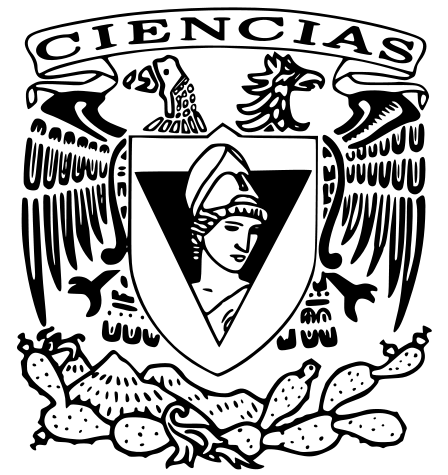
\includegraphics[scale=.19]{fac.png}}
\end{picture}

\begin{center}
\vspace*{0.2in}
{\fontsize{21}{21}\selectfont Universidad Nacional Autónoma de México}\\
\vspace*{0.2in}
{\fontsize{18}{18}\selectfont Facultad de Ciencias}\\
\vspace*{0.2in}
\begin{large}
{\fontsize{14}{14}\selectfont Laboratorio de Electromagnetismo} \\
\end{large}
\vspace*{0.2in}
\vspace*{0.2in}
\begin{Large}
\textbf{Práctica 2} \\
\textbf{Medición de la fuerza electrostática y la carga con \\ un péndulo electrostático.} \\
\end{Large}
\vspace{.7 cm}
Integrantes del equipo:\\
1) Alonso Barradas Luis Gustavo\\ 
2) Fragoso Alvarado Daniel\\ 
3) Rios Fematt Mildred Stephany\\ 
4) Robledo Ibarra Emiliano\\
\paragraph{}
\begin{figure}[H]
    \captionsetup{justification=centering,margin=2cm}
    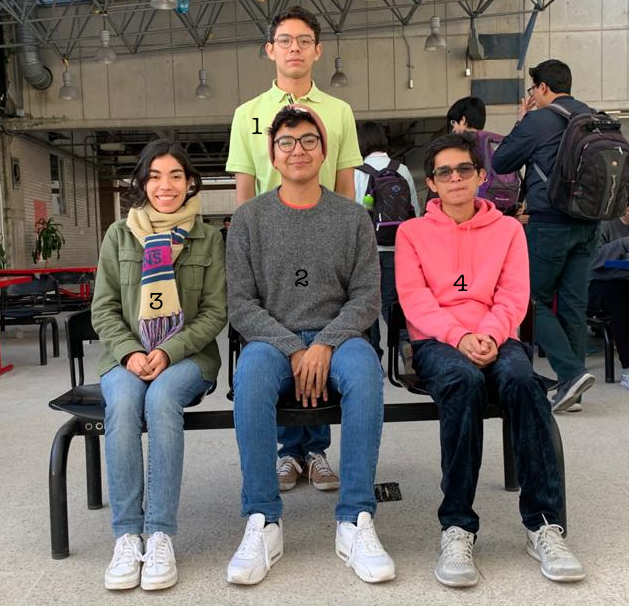
\includegraphics[scale=0.23]{uwu.jpg}
    \centering
\end{figure}
\rule{80mm}{0.1mm}\\
\begin{large}
Profesora:  Fís. Maris Sofía Flores-Cruz.  \\
Ayudante: Miguel Ángel Amaya Reyes. \\
Fecha de entrega: \today\\
\end{large}
\end{center}

\newpage

%------------------------------------

\begin{multicols*}{2}

\section{Objetivos}

\begin{enumerate}
    \item Hacer uso de un péndulo electrostático modificado con el fin de medir experimentalmente la fuerza electrostática ejercida entre dos cuerpos cargados en un sistema, debido a la inducción de cargas del mismo valor en dos cuerpos.
    \item A partir de la medición del valor de la fuerza electrostática; medir el valor de carga eléctrica en uno de los cuerpos.
    
\end{enumerate}

\section{Introducción}
%% Antecedentes históricos %%
Tras la clasificación de Benjamin Franklin sobre la existencia de dos cargas eléctricas --positiva y negativa-- varios científicos a lo largo de la década siguiente se dedicaron a tratar de hallar una relación entre estas cargas, y su interacción.

Sin embargo, no fue sino hasta 1784 que Charles Agustin de Coulomb, utilizando una balanza de torsión, pudo estudiar la fuerza de atracción entre partículas cargadas, estos cuerpos eran muy pequeños comparados con la distancia que los separaba $r$. Coulomb logró comprobar que cuando se duplicaba esta distancia $r$, la fuerza disminuía $\frac{1}{4}$ de su valor inicial, descubrió que la fuerza eléctrica es proporcional a $\frac{1}{r^2}$. Además, apoyándose en la ley de conservación de cargas, enunciada por Benjamin Franklin y William Watson, Coulomb dividió una carga en dos partes iguales poniendo en contacto un conductor esférico con carga pequeña, con una esfera idéntica pero sin carga, por la simetría, la carga se compartiría por igual entre las dos esferas \cite{resnik2002}. Agustin de Coulomb publicó sus primero 3 reportes de electricidad y magnetismo, en los cuales enunció su ley.


%% Marco Teórico $$
\textbf{Ley de Coulomb}. La ley que trata sobre la fuerza electrostática entre dos cargas se puede enunciar de la siguiente manera:

\begin{center}
    \begin{minipage}{0.9\linewidth}
        \vspace{5pt}%margen superior de minipage
        {\small
             La fuerza que actúa sobre una carga puntual fija $q_2$, debida a la presencia de otra carga puntual fija $q_1$, es directamente proporcional al producto de las cargas e inversamente proporcional al cuadrado de la distancia que las separa, está dirigida según la línea definida por ambas cargas, y es repulsiva o atractiva según sean del mismo o distinto signo las cargas.
        }
        \begin{flushright}
            (Alonso, et. al., 1999, p. 460)
        \end{flushright}
        \vspace{5pt}%margen inferior de la minipage
    \end{minipage}
\end{center}

Matemáticamente, la expresión que rige esta ley esta dada por:
\begin{equation}
   \Vec{F}_{21}=k\frac{q_1q_2}{||\Vec{r_{21}}||^2}\hat{r}_{21}
   \end{equation}
 
 donde $k$ es la \textit{Constante de Coulumb}, así $k= \frac{1}{4 \pi \epsilon_{0}}$, y donde $\epsilon_{0}$ es la \textit{permeabilidad del vacío} y para nuestros fines:

$$\epsilon_{0}= 8.854\times 10^{-12} C^2/ Nm$$
y
$$k=8.9874 \times 10^{9} Nm/ C^2$$

Observemos que la expresión matemática nos dice que las cargas iguales se repelen, y las distintas se atraen; además dicha fuerza es newtoniana, es decir $\vec{F}_{12} = -\vec{F}_{21}$.



%Además hay que considerar que la carga eléctrica esta cuantizada, la razón sigue siendo un problema por resolver, pero sabemos que esta cuantización responde a múltiplos de la carga del electrón, pues esta es la \textit{mínima} carga conocida \cite{Roller1953}.
   
\textbf{Péndulo electrostático.} El péndulo electrostático es un sistema que se utiliza para encontrar 
%QUE PEDO CON ESTO &%
el valor  de una carga y observar la interacción entre objetos cargados eléctricamente; consiste en un soporte que mantenga a un objeto colgado de él, con el fin de observar la reacción  cuando se acerca un objeto que se encuentre eléctricamente cargado; sin embargo, es posible modificar este sistema de forma que se cuelgue otro objeto y se observe la reacción al inducir alguna carga en ambos, \textbf{Figura 3}. Es posible observar que, si es el caso en el cual se le agregó un segundo objeto al sistema, éste funcionará de manera símil a un péndulo pero en este caso al existir fuerzas electrostáticas de por medio, es posible llegar a un equilibrio con ambos objetos repeliéndose mutuamente y manteniéndose en equilibrio. 

Bajo un análisis podemos observar que por la $3^{ra}$ Ley de Newton, la fuerza que ejerce $q_1$ sobre  $q_2$ es la misma que ejerce  $q_2$ sobre $q_1$ en magnitud, por lo tanto se hará el análisis para una sola esfera. \textbf{Figura 2}.

 \begin{figure}[H]
    \captionsetup{justification=centering,margin=2cm}
    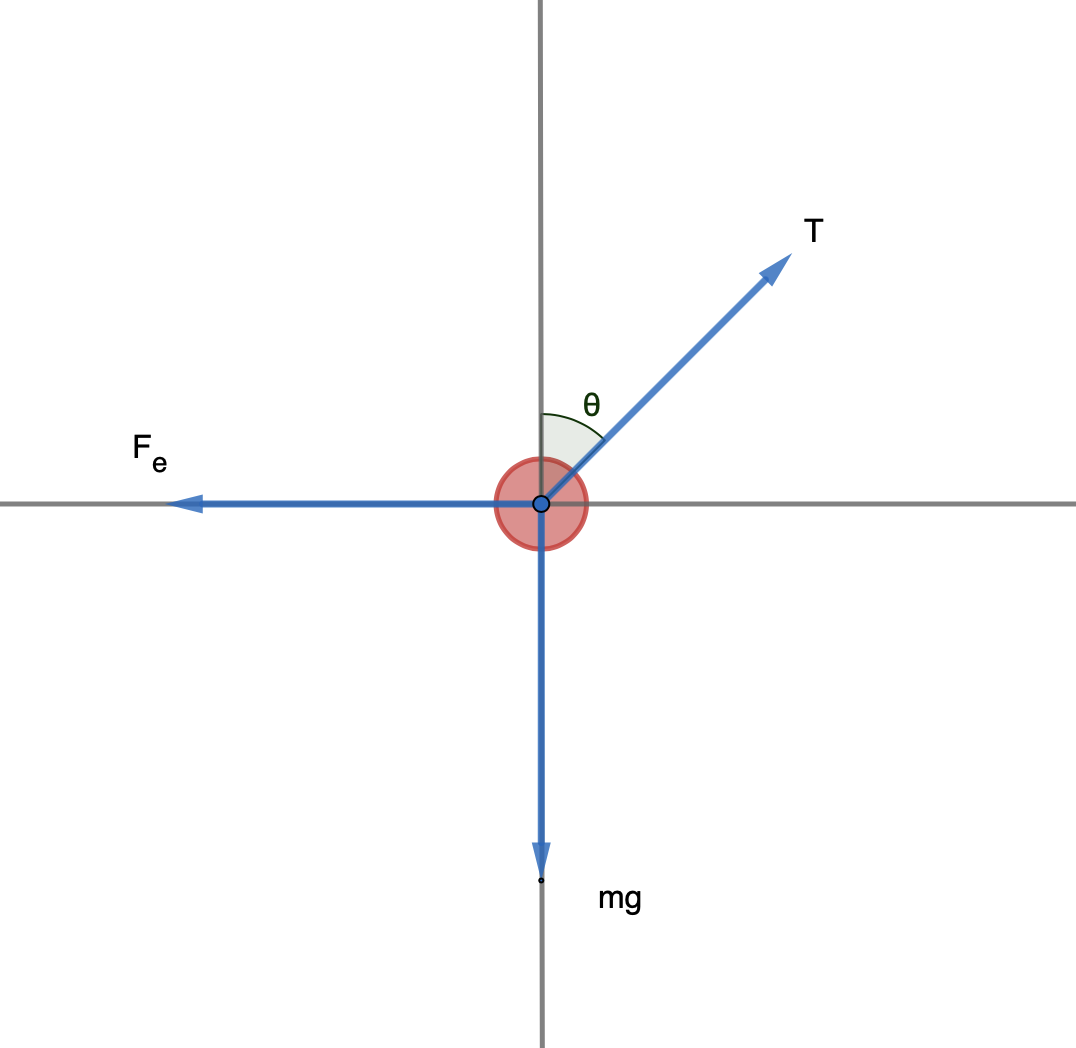
\includegraphics[scale=0.23]{pitufina.png}
    \centering
    \caption{}
\end{figure}

Bajo la suposición de que nuestro sistema está en reposo
\begin{equation*}
    \sum F_x=T\text{sin}\theta-F_e=0
\end{equation*}{}
\begin{equation*}
   \sum F_y=Tcos\theta-mg=0
\end{equation*}

Resolviendo el sistema de ecuaciones para $F_e$ 
\begin{equation}
    F_e=mg\text{tan}\theta
\end{equation}

Una vez que conocemos $F_e$ de la ecuación \textbf{(1)}, podemos calcular el valor de la carga inducida de cada esfera. Realizando un simple despeje se obtiene:

\begin{equation}
    |Q|=r\left(\sqrt{\frac{F_{e}}{k}}\right)
\end{equation}
Observemos que, matemáticamente el valor absoluto se obtiene al sacar la raíz cuadrada de un valor elevado al cuadrado. En el sentido físico, esto se refiere a que el equilibrio se dará siempre y cuando las cargas sean del mismo signo; sin importar si el sistema se cargó negativamente o postivamente. Esta carga inducida a las esferas dependió de la conexión realizada a la fuente de poder, siendo en este caso particular una inducción de carga positiva. 
\section{Desarrollo experimental}
Para este experimento se dispuso de los siguientes materiales:
%%% Lista de Materiales %%%
\setlist{nolistsep}
\begin{itemize}
    \item Soporte universal
    \item Dos varillas de nylon
    \item Nuez
    \item Hilo no conductor
    \item Esferas de unicel
    \item Balanza Scout® Pro Balance ($\pm 0.01$g).
    \item Fuente de poder de alta tensión DC: 0...25 kV PHYWE (+6\%/-10\%)
    \item Papel aluminio
    \item Cámara de video 
\item Flexómetro ($\pm0.0005m$)
\end{itemize}{}
%%%%%%%%%%%%

A continuación se muestra un diagrama del sistema que se utilizó para las obtenciones de las mediciones utilizadas:


 \begin{figure}[H]
    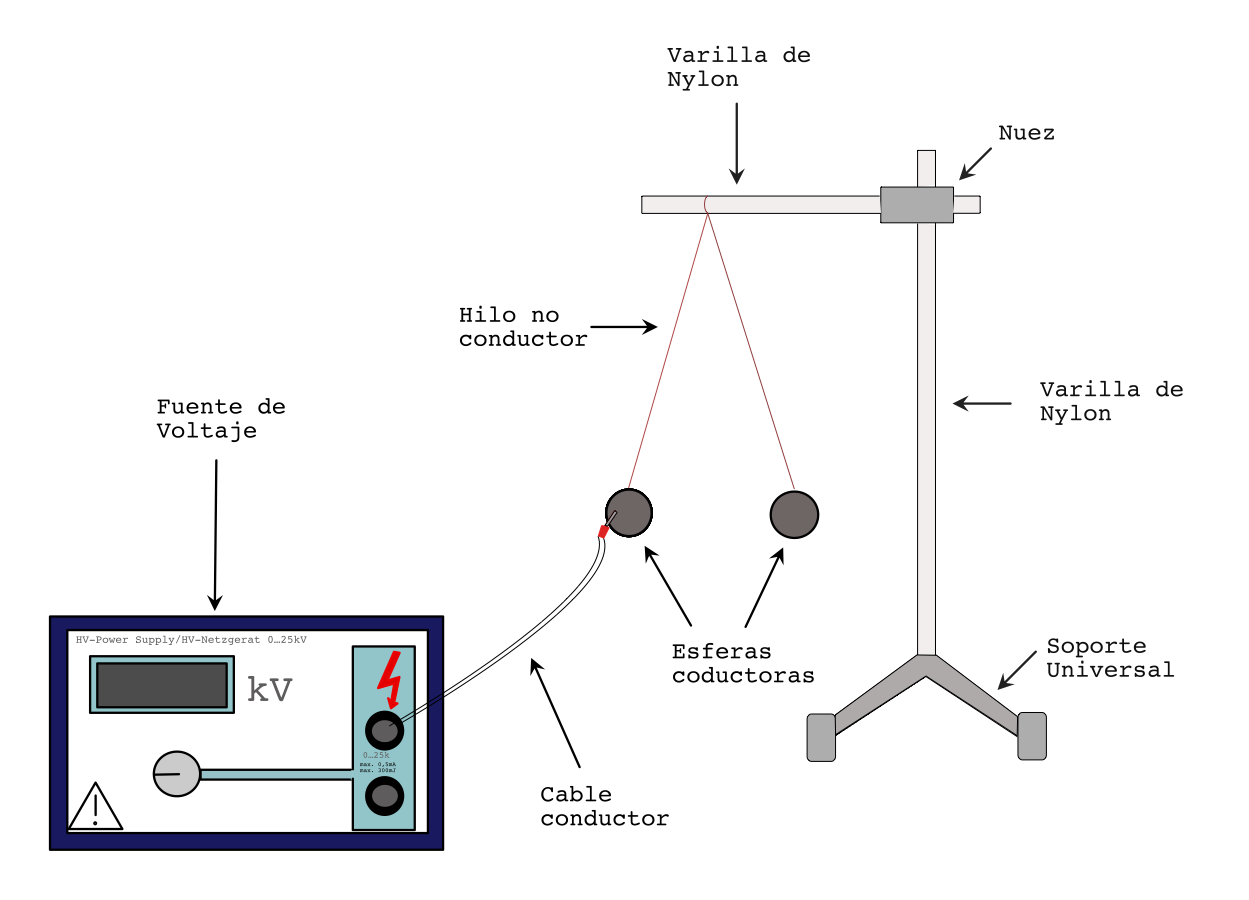
\includegraphics[scale=0.19]{turbomamalon.png}
    \centering
    \caption{Esquema del Arreglo experimental.}
\end{figure}

%%%%%%%%%%%


%%% Descripción del Montaje %%%
Se procedió a montar sobre un soporte universal una varilla de nylon, a la cual se le colocó una nuez para poder agregar una segunda varilla. De esta última varilla fueron colgados dos hilos atados al mismo nodo; de los cuales pendían dos esferas de unicel envueltas en papel aluminio.
Originalmente las esferas presentaban pintura conductora en su superficie; sin embargo, al momento de realizar el experimento se encontró que se tenía una mejor repulsión entre ellas al estar envueltas en aluminio. Aunado a esto, las esferas por sí solas contaban con una masa distinta; es por ello que, al haber sido envueltas en aluminio, se pudo contar con dos esferas igualadas en masa y prácticas, en comparación de las esferas solas, para la realización del experimento, véase (\textbf{Figura 3}).
 
Una vez montado el péndulo electroestático, fue colocado un tipo de barrera que evitaría que el sistema rotase. Sencillamente se colocó una hoja sobre la parte posterior de la mesa, de manera que hiciera presión sobre los hilos, provocando que éstos no rotaran, y sin evitar que siguieran su movimiento de traslación. A pesar de que sabíamos que esto agregaría una variable extra en nuestro análisis, que es la fuerza de fricción producida por la hoja, consideramos que poder disminuir la rotación era más conveniente para nuestro análisis y se podría despreciar esta fuerza, dado que la parte que rozaba el hilo con la hoja era una superficie pequeña, para así llegar al sistema en equilibrio que se propuso desde un inicio. 

Por último, para poder cargar las esferas por el método de electrización por contacto, se empleó una fuente de voltaje, conectando a ella un cable conductor y luego acercándolo a una de las esferas. Véase \textbf{Figura 3}.

%%%%%%%%%

 \begin{figure}[H]
    \captionsetup{justification=centering,margin=0cm}
    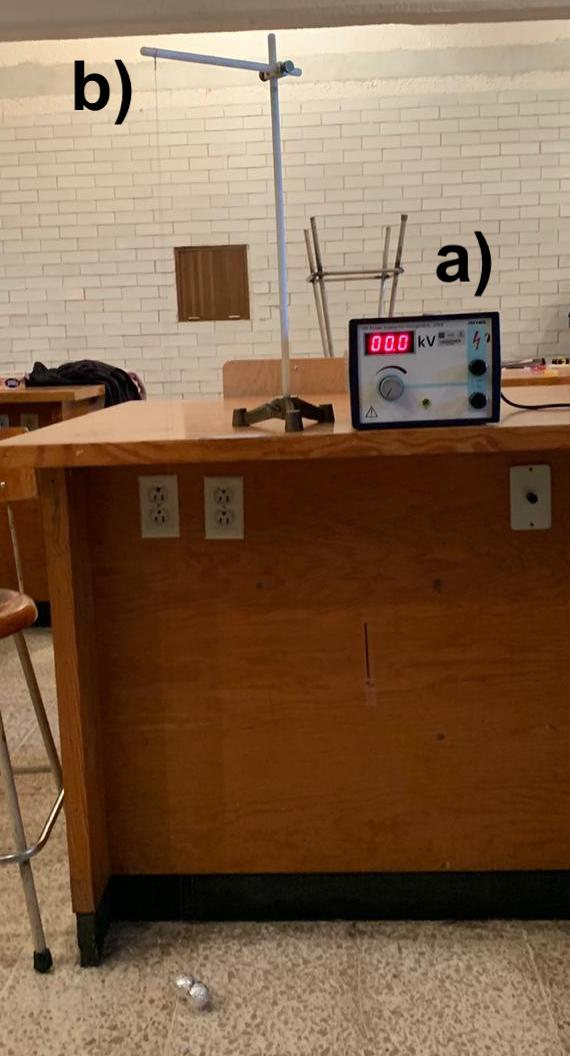
\includegraphics[scale=0.23]{pitillino.jpeg}
    \centering
    \caption{Diseño Experimental: a)Arreglo experimental, soporte universal con dos esferas, b) Fuente de Voltaje.}
\end{figure}

%%%%%%%%


%%% Descripción del Proceso de Medición %%%
 
Una vez conectada la fuente de poder, se estabilizaron ambas pelotas de unicel de manera que se evitase su rotación por medio de la barrea previamente colocada. Al mismo tiempo, fue colocada en la mesa una referencia de longitud, pegando cinta adhesiva y marcando una longitud de 10 cm, la cual se utilizaría como vara de calibración al momento de realizar el análisis por medio del software Tracker. De igual forma, para obtener una incertidumbre similar en las 5 mediciones, se colocó una referencia en el piso que indicaba desde dónde fue colocada la cámara para poder grabar el efecto que ocurría al inducir las cargas a ambas esferas.

Posteriormente, para una misma longitud $L=(1.160 \pm 0.005)$ m , que permaneció constante, se cambió el voltaje de manera que se obtuvieron cinco mediciones distintas de las distancias entre las esferas, como resultado de inducir una carga al sistema.
Los diferentes videos obtenidos fueron analizados con ayuda de Tracker. En ellos se obtuvo una distancia de separación entre los centros de las esferas y un ángulo de amplitud: usando la referencia a la distancia, antes mencionada, se le asoció la incertidumbre $\pm 0.05$ m obtenida mediante un equivalencia entre distancias (\textbf{Apéndice 1}). En el caso del ángulo, se supuso un triángulo isósceles, sabiendo que a la mitad de la distancia podemos hacer un triángulo rectángulo con hipotenusa $L$ (longitud del hilo) y como base la distancia obtenida entre dos; usando la función $arcsin(r/2L)$ se encontró el ángulo utilizado, y su incertidumbre dada por la propagación de incertidumbres.


%Usando la ecuación \textbf{(3)} y una vez calculada la magnitud de la fuerza eléctrica, se obtiene el valor de la carga inducida a las esferas en cada voltaje distinto y la incertidumbre que se le asoció se obtuvo mediante la propagación de incertidumbres (ver \textbf{Apéndice}).


\section{Resultados, análisis y discusión}

Para la longitud del hilo se eligió arbitrariamente su longitud de $L = (1.160 \pm 0.005)$m. La masa de las esferas, después de haber sido igualadas, fue $m = (0.28\pm 0.01)g$. Para la misma longitud $L$ se usaron los siguientes voltajes y se analizó la fuerza eléctrica entre ellos:

\begin{itemize}
    \item $V_1=(14.1 +0.8/-1.4) kV$.
    \item $V_2=(15.1 +0.9/-1.5) kV$.
    \item $V_3=(16.6 +1.0/-1.7) kV$.
    \item $V_4=(20.5 +1.2/-2.0) kV$.
    \item $V_5=(25.0 +1.5/-2.5) kV$.
\end{itemize}

En el primer voltaje, $V_1=(14.1 +0.8/-1.4) kV$, se obtuvo un valor de fuerza de:
\begin{equation*}
    F_e= ( 9\times 10 ^{-5} \pm  7\times 10 ^{-5})N  
\end{equation*} 
donde $ \theta =( 0.03 \pm 0.02) $ rad, que es la mitad del ángulo entre los hilos.

Para el siguiente voltaje,  $V_2=(15.1 +0.9/-1.5) kV$, el valor de la fuerza obtenido fue:
\begin{equation*}
    F_e= ( 9\times 10 ^{-5} \pm  7\times 10 ^{-5})N  
\end{equation*} 
siendo $ \theta =( 0.03 \pm 0.02) $ rad   la mitad del ángulo entre los hilos.

Con el voltaje  $V_3=(16.6 +1.0/-1.7) kV$ se calculó un valor de fuerza de:
\begin{equation*}
    F_e= ( 9\times 10 ^{-5} \pm  7\times 10 ^{-5})N  
\end{equation*} 
con $ \theta =( 0.03 \pm 0.02) $ rad  como  la mitad del ángulo entre los hilos.

En el cuarto voltaje, $V_4=(20.5 +1.2/-2.0) kV$ se obtuvo un valor para la fuerza de:
\begin{equation*}
    F_e= ( 1.0\times 10 ^{-4} \pm  0.7\times 10 ^{-4})N  
\end{equation*} 
donde $ \theta =( 0.04 \pm 0.02) $ rad  es la mitad del ángulo entre los hilos.

Para el 5to y último voltaje dado,  $V_5=(25.0 +1.5/-2.5) kV$,  el valor de la fuerza eléctrica fue:
\begin{equation*}
    F_e= ( 1.5\times 10 ^{-4} \pm  0.8\times 10 ^{-4})N  
\end{equation*} 
con  $ \theta =( 0.05 \pm 0.02) $ rad  como  la mitad del ángulo entre los hilos.

Dadas las fuerzas calculadas se tienen los siguientes valores de carga gracias a la ecuación \textbf{(3)}:

\begin{itemize}
\item  $Q_1 =( 5\times 10^{-9} \pm 5\times 10^{-9}) C$
\item  $Q_2 =( 6\times 10^{-9} \pm 5\times 10^{-9}) C$
\item  $Q_3 =( 6\times 10^{-9} \pm 6\times 10^{-9}) C$
\item  $Q_4 =( 7\times 10^{-9} \pm 2\times 10^{-9}) C$
\item  $Q_5 =( 8\times 10^{-9} \pm 2\times 10^{-9}) C$
\end{itemize}

Donde $Q_1$ es la carga inducida por la fuente de voltaje con un valor de $V_1=(14.1 +0.8/-1.4) kV$; $Q_2$ es la carga inducida por un valor de voltaje $V_2$; y así sucesivamente.  



Al calcular la magnitud de la fuerza eléctrica entre las esferas, se obtuvieron distintos valores de la misma; ya que como se pudo observar en la ecuación \textbf{(2)}, tal magnitud depende del ángulo; y como ya se mencionó, éste fue calculado de forma indirecta. Dado que muchas veces fue complicado encontrar al sistema en equilibrio, se tomó en cuenta la distancia dónde las esferas permanecieron en reposo durante mayor duración de tiempo, a la par, se pudo observar que entre más voltaje se inducía, las esferas solían separarse más.

La relación de ambos resultados se asocia a la definición de Fuerza eléctrica \textbf{(1)}, la cual indica su dependencia directa con el valor de las cargas. Por lo tanto, al presenciar una mayor carga en las esferas se produjo una fuerza de repulsión mayor ente ellas, dando como resultado un alejamiento significativo en comparación de las cargas menores. 

Es importante marcar que esta dependencia de la fuerza con las cargas de las esferas se hizo más notorio al aplicar distintos voltajes a las esferas. Conforme éste último iba en aumento, la fuerza calculada fue cada vez mayor. 
En seguida se muestran las distancias entre las esferas para cada voltaje distinto:

\begin{itemize}
\item $r_1= (5.40\times 10^{-2}\pm0.05\times 10^{-2} )m$
\item $r_2= (5.59\times 10^{-2}\pm0.05\times 10^{-2} )m$
\item $r_3= (5.75\times 10^{-2}\pm0.05\times 10^{-2} )m$
\item $r_4= (5.93\times 10^{-2}\pm0.05\times 10^{-2} )m$
\item $r_5= (6.18\times 10^{-2}\pm0.05\times 10^{-2} )m$
\end{itemize}

donde, $r_1$ es la distancia entre las esferas después de haberles aplicado un voltaje $V_1$; $r_2$ al haberse aplicado un voltaje $V_2$; y así sucesivamente. 

De los datos anteriores se puede apreciar el efecto de repulsión para cada distinto voltaje aplicado; y cómo, al ir éste en aumento, la distancia, como producto de repulsión entre las esferas, fue a su vez en aumento.

Se obtuvo el valor de la fuerza eléctrica generada por carga inducida a las esferas y, como consecuente de esto, se pudo obtener el valor de la carga inducida. Todo derivado de la dependencia de la fuerza con la carga, pero quedando en remanencia el por qué las cargas eventualmente se disminuían conforme pasaba el tiempo durante el análisis del sistema. Se conoce que la carga se mantiene constante en un sistema aislado, dado que en nuestro sistema sabemos que existe una disminución en la distancia de separación entonces podemos pensar en una disminución de la fuerza eléctrica y que esta disminución es derivada de una pérdida en las cargas; además de la notoria variación en las separaciones, conocemos que el aire es ionizable; de manera que al inducir una carga en un material en contacto con el aire, se pueden compartir con aquel esta carga inducida: es así como una carga inducida comienza a transferirse a otros materiales que lo rodean, de manera que la carga en un cuerpo no permanece constante sino que va intercambiándose con el sistema.
Aunado a esto, se observó que aumentar el voltaje generado por la fuente daba como resultado un mayor alejamiento de las esferas y una amplitud mayor en cuanto al ángulo de separación. Lo anterior se puede traducir en que un aumento en el voltaje implica una mayor carga en las esferas por lo cual una fuerza eléctrica de magnitud más grande y por lo tanto la distancia entre estas esferas aumenta.

En cuanto a los valores que se obtuvieron respectivos a la fuerza eléctrica estos resultan tener asociados de por medio incertidumbres porcentuales entre 53\% y 78\% los cuales provienen de la forma de medir ángulos asociados a cada voltaje inducido, y como estos tienen incertidumbres asociadas con porcentajes similares, basándonos en este hecho no sólo podemos ver que la forma de medición fue incorrecta, sino que resulta perfectible y que debido a este error los valores de las cargas que se obtuvieron resultaron inútiles puesto que la incertidumbre con la cual cuentan tienen valores casi iguales a su medida. A pesar de haber medido tanto la fuerza eléctrica como el valor de la carga utilizando las ecuaciones teóricas, no es posible afirmar si los valores son los que se reportan en la teoría, la dificultad adviene en el hecho de que la única medida confiable, en el sentido de que su incertidumbre es lo suficientemente pequeña comparada a su valor, es la distancia de separación entre los centros de las esferas y tanto la fuerza, la carga y los ángulos no son para nada fiables.





\section{Conclusiones}

Se dispuso de un péndulo electrostático ensamblado con material de laboratorio cuya principal función recayó en ayudar a notar con claridad los efectos producidos por las fuerzas eléctricas ejercidas por las esferas, una vez que fue inducida a ambas gracias a la fuente de voltaje la cual proporcionó carga a las esferas; sin embargo, se sabe que la variación de este experimento con el que utilizó Coulomb, fue una balanza de torsión; dando una mayor precisión al momento de calcular la distancia de separación. Además el método de carga en las esferas fue el de carga por contacto. Como únicamente fue inducida carga a una esfera con un cierto voltaje, ésta misma al estar en contacto con la otra le proporcionó cierta carga hasta poseer una carga de valor similar, dando posibilidad a errores sistemáticos, como lo son, el proporcionar cierto movimiento adicional a las esferas.

Algunos de los problemas que se presentaron al calcular la fuerza eléctrica recaían en nuestras hipótesis principales: la primera, el hecho de suponer que $r << R$, donde $r$ es el radio de las esferas y $R$ la distancia de separación entre éstas; lo cual a grandes rasgos, no se cumplía. Lo segundo, fue suponer un sistema en equilibrio. Al momento en que nosotros cargábamos las esferas, había veces dónde les era agregada cierta cantidad de movimiento, esto, junto con la fuerza eléctrica de repulsión, ocasionaba que las esferas no lograran el equilibrio buscado; sino que, la inercia provocaba que éstas chocaran unas contra otras, o incluso presentándose veces que en que comenzaban a rotar.


Como objetivo de la práctica se buscaba obtener una descripción de la Ley de Coulomb; y tal y como se había reportado en la literatura, pudimos ver que aunque al aplicar un gran voltaje a cada esfera, éstas no obtuvieron mucha carga, lo cual era de esperarse, porque para dar un parámetro de referencia, la fuerza eléctrica que separa a dos protones es un aproximado de $10 ^{36} $ veces más grande que la gravitatoria, si hubiéramos obtenidos valores de carga más grandes, esto hubiera implicado que nuestra fuerza hubiera sido sumamente mayor, con la posibilidad de romper el hilo. 
En cuanto a los valores de la fuerza, a pesar de haber reportado los resultados obtenidos en cifras significativas, estas cifras mostraban un pequeño incremento  por cada incremento de voltaje, que nos indica de la relación directa de las cargas con la fuerza, dándonos así una descripción cualitativa de cómo se comporta la fuerza eléctrica entre dos cuerpos .

Como último punto, es necesario mencionar los problemas que resultaron de las mediciones y las correcciones propuestas para la obtención de datos. Durante las mediciones, las esferas rotaban y los hilos del péndulo se entrelazaron uno con otro; lo cual es evitable con longitudes de hilo más pequeñas. Los ángulos medidos formaron parte fundamental para el cálculo de la fuerza eléctrica; sin embargo, se requiere una forma distinta de medición que sea más sensible, como grabar el nodo del cual penden ambas esferas y registrar dichas inclinaciones. En cuanto al intercambio de cargas que sabemos que ocurre, podría aislarse el sistema de manera que el aire sea mínimo o al menos no esté en constante flujo y su pérdida sea mínima con el exterior.

\nocite{*}
\bibliographystyle{apacite}
\bibliography{mybib}



\appendix
\section{Anexo I}

En esta sección se añaden los cálculos propios a las incertidumbres asociadas en las mediciones realizadas, para ello se requirió de la ecuación de propagación de incertidumbres por medio de suma de cuadrados \cite{beving}.

Para obtener la incertidumbre asociada a Tracker, de acuerdo a nuestra vara de calibración, en cada grabación se puso como referencia una línea que media 10 cm, para cada video se tomó el número de pixeles contenidos en 10 cm y mediante una regla de 3, se obtuvo la mínima medida que Tracker podía tomar, para así asociarle a la mitad de esta cifra, la incertidumbre de la medida
$$\sigma_x=\frac{(1\textit{pixel})0.1m}{2\# pixeles}$$

De la ecuación (1) y utilizando la ecuación de propagación de incertidumbres obtenemos la incertidumbre asociada a la fuerza eléctrica calculada:
\begin{equation}
    \sigma_{F_e}=\sqrt{\left(\sigma_m \frac{\partial F_e}{\partial m}\right)^2+\left(\sigma_\theta \frac{\partial F_e}{\partial \theta}\right)^2}
    \end{equation}
donde las derivadas parciales son \begin{equation*} 
\begin{split}
\frac{\partial F_e}{\partial m} &=g \text{tan}\theta \\  
\frac{\partial F_e}{\partial \theta}&=mgsec^2\theta 
\end{split}
\end{equation*}

Y las incertidumbres de las medidas de
%%%%
%Cálculos mamones
%%%%
De la ecuación (3) podemos utilizar su ecuación de propagación de incertidumbres de la forma:
\begin{equation}
     \sigma_{q}=\sqrt{\left(\sigma_r \frac{\partial q}{\partial r}\right)^2+\left(\sigma_{F_e} \frac{\partial q}{\partial F_e}\right)^2}
\end{equation}{}
donde las derivadas parciales son: \begin{equation*} 
\begin{split}
\frac{\partial Q}{\partial r} &=\sqrt{\frac{F_e}{k}} \\  
\frac{\partial Q}{\partial F_e}&=\frac{r}{2\sqrt{kF_{e}}} 
\end{split}
\end{equation*}
Y las incertidumbres de $r$ y $F_e$ son las antes mencionadas.

Análogamente, para encontrar la incertidumbre del ángulo se utilizo la misma ecuación
\begin{equation}
     \sigma_{\theta}=\sqrt{\left(\sigma_r \frac{\partial \theta}{\partial r}\right)^2+\left(\sigma_L \frac{\partial \theta}{\partial L}\right)^2}
\end{equation}
donde las derivadas parciales son: \begin{equation*} 
\begin{split}
\frac{\partial \theta}{\partial r}
&=\frac{1}{\sqrt{4L^2-r^2}} \\  
\frac{\partial \theta}{\partial L}&=-\frac{r}{L\sqrt{4L^2-r^2}} 
\end{split}
\end{equation*}


\end{multicols*}

\end{document}